% small.tex
\documentclass{beamer}
%include polycode.fmt
\usepackage{xcolor}
\usepackage{media9}
\usepackage{tikz}
\usetikzlibrary{patterns}
\usepackage{pgfplots}
\usepackage[normalem]{ulem}
\usepackage{color, colortbl}
\usepackage{tikz}
\usetikzlibrary{trees}
\usetikzlibrary{shapes}
\definecolor{green}{rgb}{0,1,0}
\definecolor{navyblue}{rgb}{0.2,0.2,0.7}
\usetheme{Antibes}
\useoutertheme[subsection=false]{miniframes}
\usenavigationsymbolstemplate{}
\newsavebox\MBox
\newcommand\Cline[2][red]{{\sbox\MBox{$#2$}%
  \rlap{\usebox\MBox}\color{#1}\rule[-1.2\dp\MBox]{\wd\MBox}{0.5pt}}}
  
\title{Monadic Functional Reactive Programming}
\author{Atze van der Ploeg}
\institute{
Centrum Wiskunde \& Informatica, Amsterdam, The Netherlands}

\newcommand{\dfcode}[1]{\begin{flalign*}\vspace{-0.35cm}#1\vspace{-0.35cm}\end{flalign*}}
\newcommand{\mul}{\!\times\!}
% \date{\today}
\begin{document}

% \AtBeginSection[]
% {
%    \begin{frame}
%        \frametitle{Outline}
%        \tableofcontents[currentsection]
%    \end{frame}
% }


%--- the titlepage frame -------------------------%

\begin{frame}[plain]
\begin{center}
  \scalebox{12}{$\bind$}
\end{center}
\vspace{-0.5cm}
  \titlepage
\end{frame}

\section{Intro}
%format =~ = "\approx"
%format ... = "\dots"
\begin{frame}{Transformational vs. Reactive}
\begin{block}{Transformational program}
|TransformationalProgram =~ Input -> Output|\\
Examples: \begin{itemize}
\item Traditional compiler
\item Compute math expression
\end{itemize}
\end{block}
\begin{block}{Reactive program}

|ReactiveProgram =~ Event -> (Output, ReactiveProgram) |
Examples: \begin{itemize}
\item IDE
\item Spreadsheet
\item Any program with GUI
\end{itemize}
\end{block}
\end{frame}

\begin{frame}{* The problem}


\begin{block}{What does this do?}
\tiny
\begin{verbatim}
class ANotifier implements
      MouseListener, TimeListener 
      extends Notifier{

  boolean first;

  ANotifier(){
   mouse.registerMouseListener(this);
   first = true;
  }

  void mouseClicked(Event e){
   if(e.but == RIGHT_BNT) {
     if(first){
       timer = new Timer(0.2);
       timer.registerTimeListener(this);
     } else {
       timer.stop();
       notifyListeners();
     } 
   }

   void timeElapsed(Event e){
     first = true;
   }
}
     

\end{verbatim}

\end{block}
\end{frame}


\begin{frame}{* The problem}
\begin{tabular}{l l}
 \begin{minipage}[t]{0.45\textwidth}
\begin{block}{What we mean}
\only<1>{
\tiny
\begin{verbatim}
wait for double right click =
  wait for right click 
  if right click within 200 miliseconds 
  then done
  else restart
\end{verbatim}
}
\only<2>{
\tiny
\begin{code}
doubler = 
  do  rightClick
      r <- rightClick `before` sleep 0.2
      if r then return () else doubler
\end{code}
}
\end{block}
\end{minipage}

& 
 \begin{minipage}[t]{0.45\textwidth}

\begin{block}{What we say}
\tiny
\begin{verbatim}
class DblRCNotifier implements
      MouseListener, TimeListener 
      extends Notifier{

  boolean first;

  DblRCNotifier(){
   mouse.registerMouseListener(this);
   first = true;
  }

  void mouseClicked(Event e){
   if(e.but == RIGHT_BNT) {
     if(first == true){
       timer = new Timer(0.2);
       timer.registerTimeListener(this);
     } else {
       timer.stop();
       notifyListeners();
     } 
   }

   void timeElapsed(Event e){
     first = true;
   }
}
     

\end{verbatim}

\end{block}
\end{minipage}
\end{tabular}
\end{frame}

\newcommand{\inlineitem}{%
{\color{navyblue} \leavevmode\usebeamertemplate{itemize item} }
}
\begin{frame}{What is unique about reactive programming?}
\begin{block}{Reactive programming means...}
Dealing with external events which may occur in \alert{in any order}.\\
\vspace{0.2cm}
Traditional approaches:\\
\begin{tabular}{l l l}
\inlineitem & Concurrency &\only<2->{$\rightarrow$ non-determinism}\\
\inlineitem & Blocking I/O multiplexing &\only<2->{$\rightarrow$ non-composable}\\
\inlineitem & Callbacks (observer pattern) & \only<2->{$\rightarrow$ inversion of control} \\
\end{tabular}
\end{block}
\only<3>{
\begin{block}{Functional reactive programming}
Functional ways of programming reactive system, which are \alert{deterministic}, \alert{composable} and \alert{without inversion of control}.
\end{block}
}

\end{frame}
    




\begin{frame}{What is Monadic FRP?}
\begin{block}{Monadic FRP is ...}
\begin{enumerate}
\item A novel monadic programmer interface for FRP
\item A novel evaluation mechanism for FRP

\end{enumerate}
\end{block}
\end{frame}

\begin{frame}{* What the hell is a Monad anyway?}

\begin{itemize}
\item Interface for composing ``steps''
\item ``Programmable semicolon''
\item Functional design pattern
\item ``Is a monad'' means implements the monad interface
\pause
\item ... just a monoid in the category of endofunctors
\end{itemize}



\end{frame}

\begin{frame}{* How i learned to stop worrying and accept monads }
\begin{block}{Formal stuff}
\begin{code}
class Monad m where
  return   :: a -> m a
  (>>=)  :: m a -> (a -> m b) -> m b
\end{code}
\end{block}
Example: Imperative looking I/O
\begin{code}
return  :: a     -> IO a
(>>=)   :: IO a  -> (a -> IO b) -> IO b
read    :: IO String
write   :: String -> IO ()
\end{code}
\vspace{-0.8cm}
\only<1>{
\begin{code}
concatInp :: IO ()
concatInp =  read >>= (\x -> 
             read >>= (\y ->
             write (x ++ y)))
            

\end{code}
}
\only<2>{
\begin{code}
concatInp :: IO ()
concatInp =  read >>= \x -> 
             read >>= \y ->
             write (x ++ y)
\end{code}
}
\only<3>{
\begin{code}
concatInp :: IO ()
concatInp = do  x <- read  
                y <- read
                write (x ++ y)
\end{code}
}

\end{frame}


\begin{frame}{* How i learned to stop worrying and love monads }

Example: LL parsing 
\begin{code}
return     :: a     -> ParserOf a
(>>=)      :: ParserOf a  -> (a -> ParserOf b) -> ParserOf b
readInt    :: ParserOf Int
eat        :: Char -> ParserOf ()
runParser  :: ParserOf a -> String -> Maybe a
\end{code}
\vspace{-0.5cm}
\begin{code}
parseTriple :: ParserOf (Int,Int,Int)
parseTriple = do  eat '(' 
                  a <- readInt  
                  eat ','
                  b <- readInt
                  eat ','
                  c <- readInt
                  eat ')'
                  return (a,b,c)
\end{code}


\end{frame}



\section{Programmer interface}

\begin{frame}{Reactive computations}

\begin{block}{Reactive computation}
A monadic computation which may require the occurrence of external events to continue
\end{block}
\vspace{-0.3cm}
\begin{code}
data R ev a =~ Await (ev -> R ev a) | Done a

instance Monad (R ev) where ...
\end{code}
\vspace{-0.6cm}
\pause
\begin{block}{Example}
\vspace{-0.4cm}
\begin{code}
data GUIEv  =  MDown { but :: Int} |  ...
mouseDown :: R GUIEv Int
mouseDown = Await ( \x -> case x of  MDown i  -> Done i
                                     _  -> mouseDown)

sameClick :: R GUIEv Bool
sameClick = do  p1 <- mouseDown
                p2 <- mouseDown
                return (p1 == p2)
\end{code}
\vspace{-0.6cm}
\end{block}
\end{frame}

\begin{frame}{Parallel reactive computation composition}
\begin{block}{Parallel composition operator}
\begin{code}
race :: R ev a -> R ev b -> R ev (R ev a, R ev b)
\end{code}
Runs both reactive computations in parallel until either
completes.
\end{block}

Example: 
\begin{code}
before :: R ev a -> R ev b -> R ev Bool
before a b = do  r <- race a b
                 case r of
                   (_, Done b) -> return False
                   (Done a, _) -> return True

doubler :: R GUIEv ()
doubler = do  rightClick
              r <- rightClick `before` sleep 0.2
              if r then return () else doubler
\end{code}
\end{frame}
%format :|     = ":\!\!|\:"
\begin{frame}{Signal computations}
\begin{block}{Signal computation}
A reactive computation that may also \alert{emit} values
\begin{itemize}
\item Can \alert{end}
\item Describes the entire life time of something
\item Also a monad $\rightarrow$ composing phases
\item Defined in terms of reactive computations
\end{itemize}

\end{block}
\pause
\only<2>{
Example: Modal dialog that asks the users name
\begin{enumerate}
\item Wait for dialog to be needed
\item Emit first form of the dialog
\item Emit new forms of the dialog as the user interacts with the dialog
\item End \& return name of user
\end{enumerate}
}
\only<3>{
\begin{code} 
newtype S ev f r = ...
instance Monad (S ev f) where ...
waitFor   :: R ev r -> S ev f r
emit      :: f -> S ev f ()
\end{code}
}
\end{frame}

\begin{frame}{Example: Drawing program}
\centering
\begin{tabular}{c c}
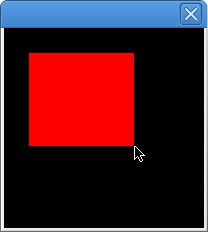
\includegraphics[width=0.3\textwidth]{01.png}
&
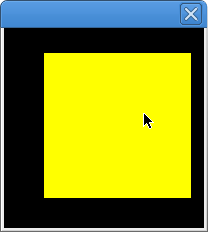
\includegraphics[width=0.3\textwidth]{02.png}
\end{tabular}
\pause
\begin{code}
type Box = (Rect,Color)
define        ::          S GUIEv Box Rect
chooseColor   :: Rect ->  S GUIEv Box Color
clickOn       :: Rect ->  R GUIEv ()
box ::  S GUIEv Box ()
box = do  r <- define
          chooseColor r
          waitFor (clickOn r)
\end{code}
\end{frame}


\begin{frame}{Another Signal computations example}
\begin{code} 
newtype S ev f r = ...
instance Monad (S ev f) where ...
waitFor   :: R ev r -> S ev f r
emit      :: f -> S ev f ()
\end{code}

Example: Cycle trough colors until right click 
\begin{code}
cycleColor :: S GUIEv Color Int
cycleColor = cc colors 0 where
   cc (h : t) i = 
     do  emit h
         r <- waitFor (middleClick `before` rightClick)
         if r then cc t (i + 1) else return i
\end{code}

\end{frame}

\begin{frame}{Dynamic lists}
\begin{tabular}{c c}
   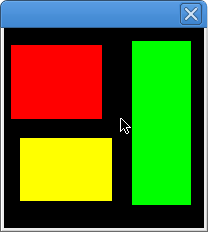
\includegraphics[width=0.3\textwidth]{05.png} &
 \begin{minipage}[b]{0.5\textwidth}
\begin{code}
box   :: S GUIEv Box ()

boxes :: S GUIEv [Box] ()
boxes = rList box

rList :: S ev f () -> S ev [f] ()

\end{code}
\end{minipage}
\end{tabular}





\begin{itemize}
\item Start a new |box| computation, and when it starts, add it to the list and repeat
\item If a |box| computation ends remove it from the list
\item If a |box| computation emits a new value update its value in the list
\end{itemize}
\end{frame}

\begin{frame}{Programmer interface summary}
\begin{block}{Reactive computations}
A monadic computation which may require the occurrence of external events to continue
\begin{code}
data R ev a =~ Await (ev -> R ev a) | Done a
instance Monad (R ev) where ...
race :: R ev a -> R ev b -> R ev (R ev a, R ev b)
\end{code}
\end{block}
\begin{block}{Signal computations}
A reactive computation that may also emit values
\begin{code}
newtype S ev f r = ...
instance Monad (S ev f) where ...
waitFor   :: R ev r -> S ev f r
emit      :: f -> S ev f ()
\end{code}
\end{block}
\end{frame}

\section{Programmer interface comparison}
%format <<< = "<\!\!\!<\!\!\!<"
%format >>> = ">\!\!\!>\!\!\!>"
%format *** = "*\!\!*\!\!*"
%format -< = "\:-\!\!\!<"
\begin{frame}{Comparison with Arrowized FRP}
Monadic FRP:
\begin{code}
cycleColor :: S GUIEv Color Int
cycleColor = cc colors 0 where
  cc (h:t) i = do
    emit h
    r <- waitFor (middleClick `before` rightClick)
    if r then cc t (i+1) else return i
\end{code}
Arrowized FRP:
\begin{code}
cycleColor :: SF MouseDown (Color, Event Int)
cycleColor = cc colors 0 where
  cc (h : t) i = switch ( proc md -> do
      mc  <- notYet <<< middleClick  -< md
      rc  <- rightClick              -< md
      returnA -< ((h,tag rc i), mc)
    ) (\ _ -> cc t (i+1))
\end{code}

\end{frame}

\begin{frame}{Comparison with Arrowized FRP}
Monadic FRP:
\begin{code}
boxes :: S GUIEv [Box] ()
boxes = rList box
\end{code}
Arrowized FRP:
\begin{code}
type BoxSF  = SF GUIIn (Box,Event ())

boxes :: SF GUIIn [Box]
boxes = boxes' [] >>> arr (map fst) where
  boxes' i = pSwitchList i
    (newBox *** arr toEv >>> arr choose >>> notYet)
    (\e l -> boxes' (mutateList e l))
choose (a,b) = merge (fmap Left a) (fmap Right b)
toEv l =  let l' = map (isNoEvent . snd) l 
          in if and l' then NoEvent else Event l'
mutate l (Left b)   = b : l
mutate l (Right l') = map fst (filter snd (zip l l'))
\end{code}
\end{frame}

\begin{frame}{Advantages \& disadvantages of Monadic FRP API}
\begin{block}{Advantages}
\begin{itemize}
\item Implicit routing
\item Sequencing phases is easier \& more intuitive
\item Easier dynamic lists 
\end{itemize}
\end{block}
\begin{block}{Disadvantages}
\begin{itemize}
\item Currently no reactive-level recursion
\item Explicit memoization needed for reactive-level sharing
\end{itemize}
\end{block}
\end{frame}

\section{Evaluation model}
\begin{frame}{Evaluation model: context}
\begin{block}{Other FRP evaluation models either ...}
\begin{itemize}
\item Re-evaluate the whole expression after each event
\item Use side-effects to prevent redundant re-evaluations
\end{itemize}
\end{block}
\pause
\begin{block}{Monadic FRP ...}
has the first \emph{purely functional} evaluation model that prevents redundant re-evaluations
\end{block}
\end{frame}

\begin{frame}{Idea}
We do not know if an event will have any effect on a reactive computation:
\begin{code}
data R ev a  =~  Await (ev -> R ev a) 
             |   Done a
\end{code}
\pause
Communicate which events a reactive computation is interested in:
\begin{code}
data R ev a  =~  Await (Requests ev) (ev -> R ev a) 
             |   Done a
\end{code}
No re-evaluation: Only call a continuation if the reactive computation is interested in the occurred event

\end{frame}

\begin{frame}{Effects on basic combinators}

\begin{itemize}
\item |a >>= b| requests the same events as |a|
\item |race a b| requests the union of the requests of |a| and |b| 
\end{itemize}
All other (Signal computation) combinators are expressed in terms of |>>=| and |race|

\end{frame}

\centering
\tikzstyle{bag} = [rectangle,text centered,draw=black,semithick,solid]
\tikzstyle{interpret} = [rectangle, rounded corners,text centered,draw=black,semithick]
 \tikzstyle{every node}=[font=\small]

\begin{frame}{Example evaluation}

\begin{tikzpicture}[grow=down, level distance=60pt]
[-]

\node[bag, name=root] {|race|}
  [sibling distance=4.5cm]
  child {node[bag] {|race|}[sibling distance=2cm]
    child {node[bag] {|mouseMove|}
       edge from parent[<-]
       node[xshift=-15pt,midway,fill=white,color=white,text=black]{$\{\mathit{MouseMove}\}$}
    }
    child {node[bag] {|mouseUp|}
       edge from parent[<-]
       node[xshift=+15pt,midway,fill=white,color=white,text=black]{$\{\mathit{MouseUp}\}$}
    }
       edge from parent[<-]
       node[xshift=-15pt,midway,fill=white,color=white,text=black]{$\{\mathit{MouseMove},\mathit{MouseUp}\}$}
       %node[left]{$\{\mathit{MouseMove},$ \\ $\mathit{MouseUp}\}$}
  }
   child {node[bag] {|>>|}  [sibling distance=2.4cm]
child {node[bag] {|mouseDown|}
       edge from parent[<-]
       node[midway,fill=white,color=white,text=black]{$\{\mathit{MouseDown}\}$}
    }
    child {node[bag] {|deltaTime|}
       edge from parent[-]
    }
       edge from parent[<-]
       node[xshift=+15pt,midway,fill=white,color=white,text=black]{$\{\mathit{MouseDown}\}$}
  }
 
 ;
\node[interpret,above of=root,yshift=+20pt,name=inter,text width=3cm] {Reactive Interpreter};
\draw [->] (root) --  (inter) node[midway,fill=white,color=white,text=black]{$\{\mathit{MouseMove},\mathit{MouseUp}, \mathit{MouseDown}\}$};
\end{tikzpicture} 
\begin{code}
race (race mouseMove mouseUp) (mouseDown >> deltaTime) 
\end{code}
\end{frame}


\begin{frame}{Example evaluation}

\begin{tikzpicture}[grow=down, level distance=60pt]
[-]

\node[bag, name=root] {|race|}
  [sibling distance=4.5cm]
  child {node[bag] {|race|}[sibling distance=2cm]
    child {node[bag] {|mouseMove|}
       edge from parent[-,dashed]
       node[xshift=-15pt,midway,fill=white,color=white,text=black]{$\{\mathit{MouseMove}\}$}
    }
    child {node[bag] {|mouseUp|}
       edge from parent[-,dashed]
       node[xshift=+15pt,midway,fill=white,color=white,text=black]{$\{\mathit{MouseUp}\}$}
    }
       edge from parent[-,dashed]
       node[xshift=-15pt,midway,fill=white,color=white,text=black]{$\{\mathit{MouseMove},\mathit{MouseUp}\}$}
       %node[left]{$\{\mathit{MouseMove},$ \\ $\mathit{MouseUp}\}$}
  }
   child {node[bag] {|>>|}  [sibling distance=2.4cm]
child {node[bag] {|mouseDown|}
       edge from parent[->,very thick]
       node[midway,fill=white,color=white,text=black]{$\{\mathit{MouseDown}\}$}
    }
    child {node[bag] {|deltaTime|}
       edge from parent[-,dashed,thin]
    }
       edge from parent[->,very thick]
       node[xshift=+15pt,midway,fill=white,color=white,text=black]{$\{\mathit{MouseDown}\}$}
  }
 
 ;
\node[interpret,above of=root,yshift=+20pt,name=inter,text width=3cm] {Reactive Interpreter};
\draw [<-,very thick] (root) --  (inter) node[midway,fill=white,color=white,text=black]{Observed: $\mathit{MouseDown}$};

\end{tikzpicture} 
\begin{code}
race (race mouseMove mouseUp) (mouseDown >> deltaTime) 
\end{code}
\end{frame}

\begin{frame}{Example evaluation}

\begin{tikzpicture}[grow=down, level distance=60pt]
[-]

\node[bag, name=root] {|race|}
  [sibling distance=4.5cm]
  child {node[bag] {|race|}[sibling distance=2cm]
    child {node[bag] {|mouseMove|}
       edge from parent[<-]
       node[xshift=-15pt,midway,fill=white,color=white,text=black]{$\{\mathit{MouseMove}\}$}
    }
    child {node[bag] {|mouseUp|}
       edge from parent[<-]
       node[xshift=+15pt,midway,fill=white,color=white,text=black]{$\{\mathit{MouseUp}\}$}
    }
       edge from parent[<-]
       node[xshift=-15pt,midway,fill=white,color=white,text=black]{$\{\mathit{MouseMove},\mathit{MouseUp}\}$}
       %node[left]{$\{\mathit{MouseMove},$ \\ $\mathit{MouseUp}\}$}
  }
   child {node[bag] {|deltaTime|}  [sibling distance=2.4cm]
       edge from parent[<-]
       node[xshift=+15pt,midway,fill=white,color=white,text=black]{$\{\mathit{DeltaTime}\}$}
  }
 
 ;
\node[interpret,above of=root,yshift=+20pt,name=inter,text width=3cm] {Reactive Interpreter};
\draw [->] (root) --  (inter) node[midway,fill=white,color=white,text=black]{$\{\mathit{MouseMove},\mathit{MouseUp}, \mathit{DeltaTime}\}$};
\end{tikzpicture} 
\begin{code}
race (race mouseMove mouseUp) deltaTime
\end{code}
\end{frame}

\begin{frame}{Why purely functional FRP evaluation matters}

Purely functional FRP evaluation $\rightarrow$ Reactive level immutability

\begin{itemize}
\item Can see different ``Futures'' \\ Examples:
\begin{itemize}
\item Duplicate drawing in drawing program into two tabs
\item Undo
\item What-if?
\end{itemize}

\item Impossible with impure evaluation model
\end{itemize}

\end{frame}
\section{Summary}

\begin{frame}{Monadic FRP: Conclusion}
\begin{itemize}
\item Programmer interface
\begin{itemize}
\item Basic concepts: Reactive \& Signal computations
\item Advantages: \begin{itemize}
\item Implicit routing
\item Sequencing phases is easier \& more intuitive.
\item Easier dynamic lists 
\end{itemize}
\end{itemize}

\item Evaluation model
\begin{itemize} 
\item First purely functional FRP evaluation model that avoids hat prevents redundant re-evaluations.
\item Purely functional FRP evaluation $\rightarrow$ Reactive level immutability
\end{itemize}

\item Future work
\begin{itemize} 
\item Implicit reactive level sharing
\item Reactive level recursion
\end{itemize}
\end{itemize}
\pause
Questions?
\end{frame}

\end{document}
